%=======================================================================
%  P2H2P wellbore primer.
%
%  Companion to notebooks/P2H2P_model.ipynb. Self-contained: one file,
%  standard packages, no external figures.
%=======================================================================
\documentclass[11pt,a4paper]{article}

\usepackage[T1]{fontenc}
\usepackage[utf8]{inputenc}
\usepackage[margin=1in]{geometry}
\usepackage{amsmath,amssymb}
\usepackage{mathtools}
\usepackage{booktabs}
\usepackage{array}
\usepackage{multirow}
\usepackage{siunitx}
\usepackage{xcolor}
\usepackage[hidelinks]{hyperref}
\usepackage{tikz}
\usepackage{pgfplots}
\pgfplotsset{compat=1.18}
\usetikzlibrary{arrows.meta,positioning,calc}

\sisetup{per-mode=symbol}
\providecommand{\celsius}{\degreeCelsius}

\newcommand{\md}{\ensuremath{\dot m}}
\newcommand{\Ui}{\ensuremath{U_{i}}}
\newcommand{\hm}{\ensuremath{h_{m}}}
\newcommand{\Tm}{\ensuremath{T_{m}}}
\newcommand{\Tpcm}{\ensuremath{T_{\mathrm{pcm}}}}
\newcommand{\Aav}{\ensuremath{A_{\mathrm{avail}}}}
\newcommand{\Amelt}{\ensuremath{A_{\mathrm{melt}}}}
\newcommand{\Elat}{\ensuremath{E'_{\mathrm{lat}}}}
\newcommand{\Eeq}{\ensuremath{E'_{\mathrm{eq}}}}
\newcommand{\Nwells}{\ensuremath{N_{\mathrm{wells}}}}
\newcommand{\epsloc}{\ensuremath{\varepsilon_{\mathrm{local}}}}
\newcommand{\code}[1]{\texttt{\small #1}}

\title{\textbf{P2H2P wellbore storage}\\[4pt]
\large A primer: how the model works\\[8pt]
\normalsize Companion to \code{P2H2P\_model.ipynb}, model version 0.6}
\author{Craft \& Hawkins Department of Petroleum Engineering\\
Louisiana State University}
\date{\today}

\begin{document}
\maketitle

\begin{abstract}
\noindent
This is a companion to the Colab notebook \code{P2H2P\_model.ipynb}: the same
material, with room to explain why each piece is the way it is. It is not the
manuscript. Nothing here is a defence of the model against a reviewer --- there
are no verification results, no comparisons with superseded formulations and no
version history. Those live in \code{P2H2P\_verification.ipynb} and in
\code{DESIGN\_NOTES.md}, and you should not need them to use or to modify the
model.

Read \S\ref{sec:overview} and \S\ref{sec:procedure} first; they are the shape
of the whole calculation. Sections \ref{sec:state}--\ref{sec:css} are the
physics, in the order the code evaluates it.
Section~\ref{sec:params} is the one to keep beside you when you start changing
things.
\end{abstract}

\tableofcontents

%=======================================================================
\section{What the plant does, and what the model computes}
\label{sec:overview}

Electricity is stored as heat and returned as electricity. During charging a
high-temperature heat pump raises heat from a warm source and delivers it to
pressurised water, which is pumped down a repurposed oil-and-gas well through
finned hairpin tubes. The annulus around those tubes is packed with a
\emph{phase-change material} (PCM), which melts and stores the energy as latent
heat. During discharging the flow reverses, the PCM freezes, and the recovered
heat drives an organic Rankine cycle (ORC) that returns electricity to the
grid. The intended duty is \SI{10}{\hour} charging and \SI{10}{\hour}
discharging, with two \SI{2}{\hour} idle periods, repeated daily.

The engineering question is how many wells a field needs to deliver a specified
electrical output --- \SI{1}{\mega\watt} here --- and what limits it.

Everything turns on one difficulty. The PCM conducts heat poorly: for the
material used here $k \approx \SI{0.5}{\watt\per\meter\per\kelvin}$, a hundred
times worse than steel. As the melt layer grows, the heat has further to travel
through a bad conductor to reach the remaining solid, so the exchanger gets
worse as it fills. A useful model must therefore couple a \emph{heat transfer
network} --- convection, tube wall, fins, and that growing melt layer --- to a
\emph{moving phase boundary}, over a duty cycle, cheaply enough to run hundreds
of times.

\paragraph{The cascade.}
One feature of this design shapes everything downstream. The water enters hot
and leaves cold: it \emph{glides} by $\Delta T_{3C,2C}=\SI{55}{\kelvin}$ along
the well. A single PCM would therefore be barely melted by the cold end of the
water and strongly superheated by the hot end. So the PCM is divided into
$N_{\mathrm{lay}}$ \textbf{layers of different melting temperature}, arranged so
that hot water meets high-melting material and cold water meets low-melting
material. Each layer sees a workable temperature difference. This is why almost
every profile in this document has a staircase in it.

%=======================================================================
\section{The calculation, end to end}
\label{sec:procedure}

Figure~\ref{fig:procedure} is the whole thing. It is worth reading before any
of the physics, because the structure is slightly unusual: \textbf{nothing is
solved for.} The thermodynamic cycles, the energy budget and the exchanger size
are evaluated in sequence; the two mass flow rates follow from prescribed
temperature glides; and the only iteration anywhere is the outer loop that
repeats the daily cycle until the store returns to its own initial state.
Section~\ref{sec:css} explains why it \emph{has} to be arranged that way.

Three levels are nested, and they are almost independent:

\begin{itemize}\itemsep2pt
\item the \textbf{plant} level --- heat pump and ORC --- is evaluated once, and
  passes only two efficiencies and a handful of water temperatures downstream;
\item the \textbf{field} level turns the \SI{1}{\mega\watt} target into an
  energy per cycle, and hence a well count;
\item the \textbf{borehole} level marches one exchanger through a half-cycle,
  and is where all the difficulty lives.
\end{itemize}

The cost is dominated by the innermost pair of loops: $n_t$ time levels
$\times$ $n_s$ segments $\times$ two half-cycles $\times$ the number of cycles
to convergence --- about $2\times10^{5}$ segment updates for the default case,
which takes a few tens of seconds.

%---------------------------------------------------------------------
\begin{figure}[p]
\centering
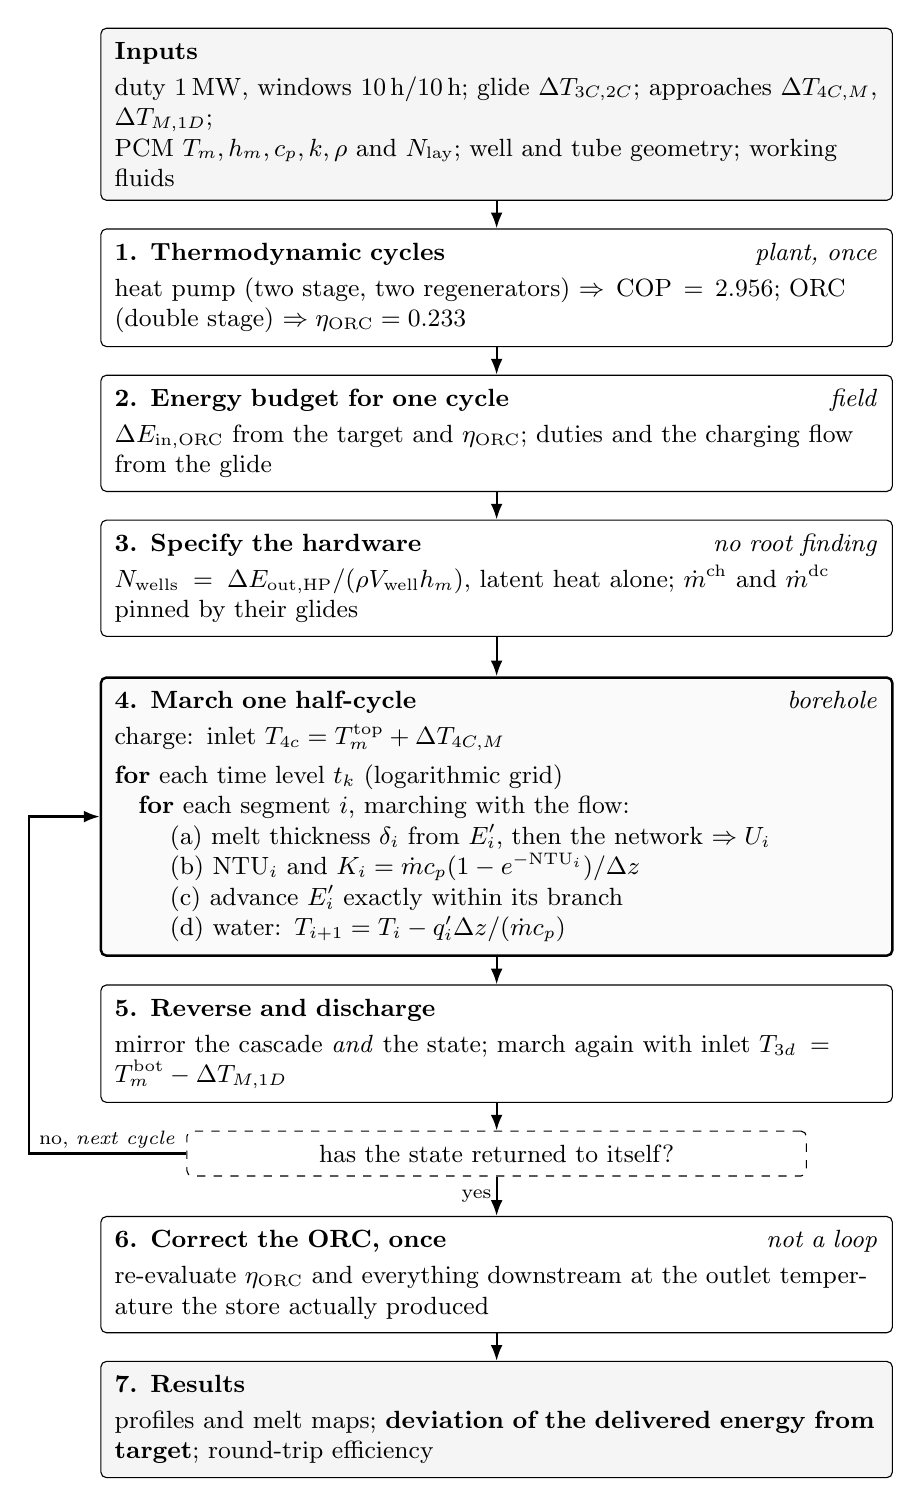
\begin{tikzpicture}[
  font=\small, node distance=3.5mm,
  blk/.style   ={draw, rounded corners=2pt, inner sep=5pt, align=left,
                 text width=0.80\linewidth},
  inp/.style   ={blk, fill=black!4},
  march/.style ={blk, line width=0.9pt, fill=black!2},
  test/.style  ={draw, dashed, rounded corners=2pt, inner sep=5pt,
                 align=center, text width=0.62\linewidth},
  fl/.style    ={-{Latex[length=2mm]}, thick},
  lab/.style   ={font=\scriptsize, inner sep=1.5pt}]

\node[inp] (in) {%
  \textbf{Inputs}\\[2pt]
  duty \SI{1}{\mega\watt}, windows \SI{10}{\hour}/\SI{10}{\hour};
  glide $\Delta T_{3C,2C}$; approaches $\Delta T_{4C,M}$, $\Delta T_{M,1D}$;\\
  PCM $\Tm,\hm,c_p,k,\rho$ and $N_{\mathrm{lay}}$; well and tube geometry;
  working fluids};

\node[blk, below=of in] (cyc) {%
  \textbf{1. Thermodynamic cycles}\hfill\emph{plant, once}\\[2pt]
  heat pump (two stage, two regenerators) $\Rightarrow \mathrm{COP}=2.956$;
  ORC (double stage) $\Rightarrow \eta_{\mathrm{ORC}}=0.233$};

\node[blk, below=of cyc] (bud) {%
  \textbf{2. Energy budget for one cycle}\hfill\emph{field}\\[2pt]
  $\Delta E_{\mathrm{in,ORC}}$ from the target and $\eta_{\mathrm{ORC}}$;
  duties and the charging flow from the glide};

\node[blk, below=of bud] (hw) {%
  \textbf{3. Specify the hardware}\hfill\emph{no root finding}\\[2pt]
  $\Nwells=\Delta E_{\mathrm{out,HP}}/(\rho V_{\mathrm{well}}\hm)$, latent heat
  alone; $\md^{\mathrm{ch}}$ and $\md^{\mathrm{dc}}$ pinned by their glides};

\node[march, below=5mm of hw] (mar) {%
  \textbf{4. March one half-cycle}\hfill\emph{borehole}\\[2pt]
  charge: inlet $T_{4c}=\Tm^{\mathrm{top}}+\Delta T_{4C,M}$\\[3pt]
  \textbf{for} each time level $t_k$ (logarithmic grid)\\
  \hspace*{3mm}\textbf{for} each segment $i$, marching with the flow:\\
  \hspace*{7mm}(a) melt thickness $\delta_i$ from $E'_i$, then the network
     $\Rightarrow \Ui$\\
  \hspace*{7mm}(b) $\mathrm{NTU}_i$ and
     $K_i=\md c_p(1-e^{-\mathrm{NTU}_i})/\Delta z$\\
  \hspace*{7mm}(c) advance $E'_i$ exactly within its branch\\
  \hspace*{7mm}(d) water: $T_{i+1}=T_i-q'_i\Delta z/(\md c_p)$};

\node[blk, below=of mar] (rev) {%
  \textbf{5. Reverse and discharge}\\[2pt]
  mirror the cascade \emph{and} the state; march again with inlet
  $T_{3d}=\Tm^{\mathrm{bot}}-\Delta T_{M,1D}$};

\node[test, below=of rev] (tst) {%
  has the state returned to itself?};

\node[blk, below=5mm of tst] (corr) {%
  \textbf{6. Correct the ORC, once}\hfill\emph{not a loop}\\[2pt]
  re-evaluate $\eta_{\mathrm{ORC}}$ and everything downstream at the outlet
  temperature the store actually produced};

\node[inp, below=of corr] (out) {%
  \textbf{7. Results}\\[2pt]
  profiles and melt maps; \textbf{deviation of the delivered energy from
  target}; round-trip efficiency};

\foreach \a/\b in {in/cyc, cyc/bud, bud/hw, hw/mar, mar/rev, rev/tst, corr/out}
  \draw[fl] (\a) -- (\b);
\draw[fl] (tst) -- node[lab,left] {yes} (corr);
\coordinate (Lx) at ($(mar.west)+(-9mm,0)$);
\draw[fl] (tst.west) -- (Lx |- tst.west)
  node[lab, midway, above] {no, \emph{next cycle}} -- (Lx) -- (mar.west);
\end{tikzpicture}
\caption{The procedure. Steps 1--3 are evaluated once and produce a fully
specified piece of hardware; steps 4 and 5 are the exchanger model, run twice
per cycle; the loop back from the test is the only iteration in the
calculation.}
\label{fig:procedure}
\end{figure}

%=======================================================================
\section{What is assumed}
\label{sec:hyp}

Every one of these is a simplification you could relax, and three of them are
worth watching in a parametric study.

\begin{center}
\begin{tabular}{@{}c p{0.42\linewidth} p{0.38\linewidth}@{}}
\toprule
 & assumption & where it bites \\
\midrule
H1 & the PCM in a segment is one lumped state & no radial temperature profile
     inside the melt \\
H2 & no axial conduction between segments & the idle periods do nothing at all \\
H3 & the melt region is a concentric annulus & \textbf{saturated} at the design
     point: neighbouring fronts touch over \SI{99}{\percent} of the well \\
H5 & one melt thickness per segment & see H1 \\
H6 & the borehole wall is adiabatic & no ground loss, so the store is lossless
     by construction \\
H7 & the water is quasi-steady & the first \SI{38}{\minute} of each half-cycle
     is not resolved \\
H8 & the cascade is laid along the developed tube length & the two legs of a
     hairpin carry different $\Tm$ at the same depth \\
H9 & no heat exchange between the two legs & they are up to
     \SI{48.9}{\kelvin} apart at the wellhead \\
\bottomrule
\end{tabular}
\end{center}

H7 deserves a sentence, because it is what makes the model cheap. The water
crosses the whole tube in \SI{2264}{\second} while the PCM state evolves over
ten hours --- a separation of about sixteen --- so the water profile is treated
as instantaneous at each time level. The price is that the startup transient of
each half-cycle is not resolved. What makes that tolerable is that the energy
held in the water is only \SI{1.2}{\percent} of the latent inventory it is
charging, so the unresolved transient misplaces very little energy even though
it occupies a noticeable fraction of the window.

%=======================================================================
\section{The state variable, and why it is enthalpy}
\label{sec:state}

Divide the developed tube length into $n_s$ segments. Each segment owns a slice
of PCM, and the model carries \textbf{one number} for it.

The obvious choice is the melt thickness $\delta$, or equivalently the melted
cross-sectional area $\Amelt$ --- it is what you would draw. It fails, for a
reason worth understanding before you trust anything else in the model.

Ask such a model for the temperature of the PCM in a segment. The only
available answer is $\Tm$: that is all the state encodes. While solid remains,
that is correct, which is why the limitation is easy to miss. It stops being
correct the moment a segment finishes melting. The network still reports a
positive heat flow --- the water is still hotter than $\Tm$, and nothing in the
resistance chain knows the PCM is exhausted --- and the model must do one of two
things. It can keep growing $\Amelt$, melting material that is not there and
producing melted fractions above unity. Or it can clip $\Amelt$ at the
available inventory and throw the surplus away, in which case the melted
fraction is physical but energy is not conserved and the water leaves at a
temperature that reflects heat which went nowhere.

Neither is acceptable, and no refinement of the marching scheme repairs either,
because the deficiency is in the \emph{state}: a variable counting melted area
has no slot for liquid above $\Tm$ or solid below it.

\paragraph{The fix.}
Carry the \textbf{enthalpy} $E'$ per unit tube length, measured from a datum of
fully solid material at that segment's own melting temperature. With $\Aav$ the
PCM cross-section belonging to one tube, define
\begin{equation}
  \Elat = \rho\hm\Aav, \qquad
  C_s = \rho c_{p,s}\Aav, \qquad
  C_l = \rho c_{p,l}\Aav,
  \label{eq:caps}
\end{equation}
the latent capacity and the two sensible capacities. The PCM temperature and
the melted area then follow from $E'$ alone:
\begin{equation}
  \Tpcm =
  \begin{dcases}
    \Tm + E'/C_s, & E' < 0 \quad\text{(subcooled solid)},\\
    \Tm, & 0 \le E' \le \Elat \quad\text{(two-phase)},\\
    \Tm + (E'-\Elat)/C_l, & E' > \Elat \quad\text{(superheated liquid)},
  \end{dcases}
  \label{eq:curve}
\end{equation}
\begin{equation}
  \Amelt = \frac{\min\bigl(\max(E',0),\,\Elat\bigr)}{\rho\hm},
  \qquad
  \epsloc = \frac{\Amelt}{\Aav} \in [0,1].
  \label{eq:amelt}
\end{equation}

Figure~\ref{fig:curve} is the reason this works. Read as $E'(T)$ the
relationship is multivalued at $\Tm$ --- which is exactly why temperature
cannot be the state variable. Read as $T(E')$, the direction used here, it is
single-valued everywhere, and position along the vertical segment \emph{is} the
melted fraction.

The saturation in Eq.~\eqref{eq:amelt} is not a guard bolted on to suppress bad
behaviour; it is the definition. Melted area saturates because a segment cannot
melt PCM it does not own, and the extra energy has somewhere to go: superheat.
So $\epsloc\in[0,1]$ is \emph{structural}. No code path can violate it and no
test for it is needed.

%---------------------------------------------------------------------
\begin{figure}[htbp]
\centering
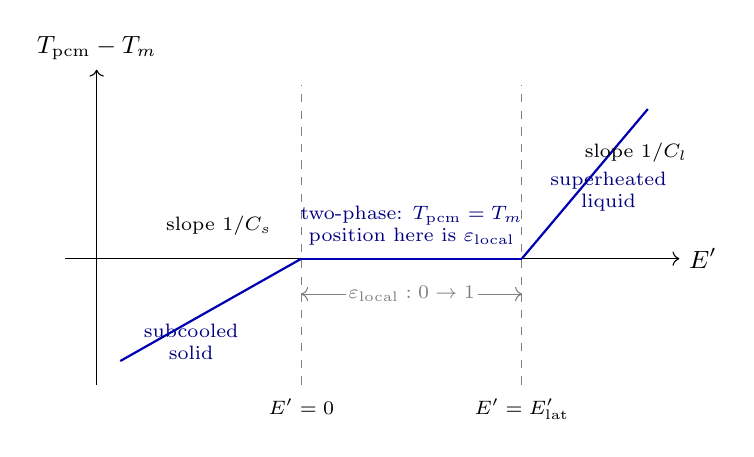
\begin{tikzpicture}[font=\small]
\draw[->] (-0.4,0) -- (7.4,0) node[right] {$E'$};
\draw[->] (0,-1.6) -- (0,2.4) node[above] {$\Tpcm-\Tm$};
\draw[thick,blue!70!black] (0.3,-1.3) -- (2.6,0);
\draw[thick,blue!70!black] (2.6,0) -- (5.4,0);
\draw[thick,blue!70!black] (5.4,0) -- (7.0,1.9);
\draw[dashed,gray] (2.6,-1.6) -- (2.6,2.2);
\draw[dashed,gray] (5.4,-1.6) -- (5.4,2.2);
\node[below,font=\scriptsize] at (2.6,-1.65) {$E'=0$};
\node[below,font=\scriptsize] at (5.4,-1.65) {$E'=\Elat$};
\node[font=\scriptsize,align=center,blue!50!black] at (1.2,-1.05)
  {subcooled\\solid};
\node[font=\scriptsize,align=center,blue!50!black] at (4.0,0.42)
  {two-phase: $\Tpcm=\Tm$\\position here is $\epsloc$};
\node[font=\scriptsize,align=center,blue!50!black] at (6.5,0.85)
  {superheated\\liquid};
\draw[<->,gray] (2.6,-0.45) -- (5.4,-0.45);
\node[font=\scriptsize,gray,fill=white,inner sep=1pt] at (4.0,-0.45)
  {$\epsloc: 0 \to 1$};
\node[font=\scriptsize] at (1.55,0.42) {slope $1/C_s$};
\node[font=\scriptsize] at (6.85,1.35) {slope $1/C_l$};
\end{tikzpicture}
\caption{The constitutive curve, Eq.~\eqref{eq:curve}. One scalar distinguishes
three physical states, and the melted fraction is where you are along the flat
part.}
\label{fig:curve}
\end{figure}

\paragraph{How much is at stake.}
It would be reasonable to guess this is a small correction. One kelvin of
superheat is worth $C_l/\Elat=c_{p,l}/\hm=\SI{0.47}{\percent}$ of the latent
capacity, so with a nominal \SI{10}{\kelvin} approach the sensible branches
look like \SI{4.7}{\percent} of the energy. The measured figure at the design
point is \textbf{\SI{9.3}{\percent}} --- \SI{7.1}{\percent} as superheat,
\SI{2.3}{\percent} as subcooling --- because \SI{10}{\kelvin} is the approach of
the \emph{first} cascade layer and a saturated segment goes on superheating past
it, reaching \SI{18.5}{\kelvin} here. And the store finishes every charge fully
molten in \emph{all} $100$ segments, so an area-based model is clipping
everywhere at the moment the store is fullest.

That number is worth recomputing whenever you change the PCM: the ratio
$c_{p,l}/\hm$ is the relevant group, so halving the latent heat doubles it.

%=======================================================================
\section{The segment equation}
\label{sec:segment}

Two control volumes, taken together: the PCM belonging to segment $i$, and the
water passing over it.

On the PCM side, all the heat arriving changes the enthalpy, by definition of
$E'$:
\begin{equation}
  \frac{\mathrm{d}E'_i}{\mathrm{d}t} \;=\; q'_i ,
  \label{eq:pcm}
\end{equation}
with $q'_i$ the heat per unit tube length crossing into the segment. On the
water side, with H7 the water carries no storage, so what it gives up is what
the PCM takes:
\begin{equation}
  T_{i+1} \;=\; T_i - \frac{q'_i\,\Delta z}{\md c_p},
  \qquad \Delta z = \frac{L_{\mathrm{tube}}}{n_s}.
  \label{eq:fluid}
\end{equation}
Marching Eq.~\eqref{eq:fluid} from the inlet gives the water profile along the
well.

What closes the pair is the relation between $q'_i$ and the temperatures. It is
tempting to write $q' = \Ui P_i (T_f - \Tpcm)$ with $\Ui$ the overall
coefficient and $P_i$ the perimeter. \textbf{That is wrong}, and in a way that
matters.

Consider what $\Ui P_i$ says as the wall conductance improves: $q'$ grows
without limit. But the water can only give up what it carries, and a segment
cannot extract more than $\md c_p$ times the temperature difference available.
Deriving the closure properly from the two balances gives the effectiveness
form,
\begin{equation}
  \boxed{\;
  q'_i = K_i\left(T_i - \Tpcm{}_{,i}\right),
  \qquad
  K_i = \frac{\md c_p\left(1-e^{-\mathrm{NTU}_i}\right)}{\Delta z},
  \qquad
  \mathrm{NTU}_i = \frac{2\pi r_i \Ui \Delta z}{\md c_p}. \;}
  \label{eq:K}
\end{equation}
As $\mathrm{NTU}\to0$ this reduces to $\Ui P_i$; as $\mathrm{NTU}\to\infty$ it
saturates at $\md c_p/\Delta z$, which is the capacity-rate limit. Over a charge
in the default case $\mathrm{NTU}$ runs from $0.083$ to $0.602$, so the two
forms differ by \SI{4}{\percent} to \SI{33}{\percent} --- largest early, when
the melt layer is thin and the exchanger is at its best.

\paragraph{Where $\Ui$ comes from.}
$\Ui$ is the usual series network referred to the inner tube area: internal
convection (Gnielinski), the fouling resistance, conduction through the tube
wall, and then the PCM side --- the finned outer surface with its fin
efficiency, in series with conduction across the annular melt layer of current
thickness $\delta_i$. That last term is the one that changes as the segment
melts, and it is what makes the problem nonlinear and interesting: the
exchanger degrades as it fills. The melt thickness is recovered from $\Amelt$
by inverting the finned-annulus area relation, which is why \code{delta\_from\_area}
exists.

%=======================================================================
\section{Integrating in time}
\label{sec:integration}

Substituting Eq.~\eqref{eq:K} into Eq.~\eqref{eq:pcm} gives, for one segment,
\begin{equation}
  \frac{\mathrm{d}E'}{\mathrm{d}t} = K\left(T_f - \Tpcm(E')\right).
  \label{eq:ode}
\end{equation}
This is nonlinear, because $\Tpcm(E')$ is piecewise --- but it is \emph{affine
within each branch} of Eq.~\eqref{eq:curve}. That structure is worth
exploiting, for a reason that is not obvious.

On the plateau, $\Tpcm=\Tm$ is constant, so the right-hand side does not depend
on $E'$ at all: the capacity is effectively infinite and explicit Euler is
\emph{exact} for any step size. On the sensible branches it is not. There
Eq.~\eqref{eq:ode} is a relaxation with time constant $C/K$, and explicit Euler
requires $\Delta t < C/K$.

The time grid here is logarithmic --- the natural choice for a diffusion-limited
process, where everything happens quickly at first and then slowly. Its last
step spans \SI{8491}{\second} against a time constant of
\SI{1102}{\second}: a ratio of $7.7$. An explicit implementation duly diverges,
and it does so spectacularly, alternating in sign and passing
\SI{8e10}{\kelvin} within twelve steps.

\paragraph{The scheme.}
Rather than refine the grid by three orders of magnitude, integrate each branch
in closed form. Holding $T_f$ fixed across the step,
\begin{equation}
  E'(t+\Delta t) =
  \begin{dcases}
    E' + K\left(T_f-\Tm\right)\Delta t, & \text{plateau},\\[4pt]
    \Eeq + \bigl(E'-\Eeq\bigr)e^{-K\Delta t/C}, & \text{sensible branches},
  \end{dcases}
  \label{eq:exact}
\end{equation}
where $\Eeq$ is the enthalpy at which the PCM would sit in equilibrium with the
water --- the state the segment relaxes toward and never reaches. The
exponential is unconditionally stable and monotone, so no step, however large,
can overshoot it. That is precisely the property explicit Euler lacks.

A step may begin in one branch and end in another, in which case it is split at
the crossing: advance to the boundary, then continue in the adjacent branch with
the remaining time. Only a few crossings can occur within one step, so the loop
is bounded.

\begin{center}
\fbox{\begin{minipage}{0.86\linewidth}\small
\textbf{One segment, one step.}
\begin{enumerate}\itemsep1pt
\item $t_{\mathrm{left}} \leftarrow \Delta t$
\item \textbf{while} $t_{\mathrm{left}}>0$:
\item \quad identify which branch contains $E'$
\item \quad compute the time $t^{*}$ to reach that branch's boundary
\item \quad \textbf{if} $t^{*}\ge t_{\mathrm{left}}$: advance by
      Eq.~\eqref{eq:exact} and stop
\item \quad \textbf{else}: move to the boundary, subtract $t^{*}$, repeat
\end{enumerate}
\end{minipage}}
\end{center}

Energy closure is then structural rather than checked: whatever the scheme puts
into $E'$ is exactly what it took out of the water.

%=======================================================================
\section{The cascade, and which temperatures you may prescribe}
\label{sec:cascade}

The layers are graded so that each sits $\Delta T_{4C,M}$ below the charging
water at \emph{its own} leading face, assuming the water glides linearly. Since
there are $N_{\mathrm{lay}}$ equal layers sharing a glide of
$\Delta T_{3C,2C}$, they are spaced one layer width apart and the coldest one is
\begin{equation}
  \Tm^{\mathrm{bot}} = \Tm^{\mathrm{top}}
   - \Delta T_{3C,2C}\,\frac{N_{\mathrm{lay}}-1}{N_{\mathrm{lay}}} .
  \label{eq:Tmbot}
\end{equation}
Note the factor $(N_{\mathrm{lay}}-1)/N_{\mathrm{lay}}$: the span of melting
temperatures is \emph{one layer width short} of the glide, because the last
layer is referenced to the water entering it rather than leaving the well. For
the default case that is \SI{48.889}{\kelvin} of cascade against a
\SI{55}{\kelvin} glide.

\paragraph{Only the inlets are boundary conditions.}
This is the single most important structural point in the model, and it is easy
to get wrong. The exchanger has two inlets and two outlets. The \emph{inlets}
are prescribed; the \emph{outlets} are computed. You cannot specify both, and
attempting to specify an outlet produces a model that contradicts itself.

\begin{equation}
  \underbrace{T_{4c} = \Tm^{\mathrm{top}} + \Delta T_{4C,M}}
    _{\text{charge: superheat, drives melting}},
  \qquad
  \underbrace{T_{3d} = \Tm^{\mathrm{bot}} - \Delta T_{M,1D}}
    _{\text{discharge: subcooling, drives freezing}}
  \label{eq:inlets}
\end{equation}

Why it matters: under Eq.~\eqref{eq:curve} the store finishes each charge
superheated, so the water leaving at the start of the next discharge is at
\SI{157.93}{\celsius} --- \emph{above} the melting temperature of the hottest
layer. Any prescribed value for that outlet is contradicted by the solution
itself. The outlet is a result, and it is reported as one.

\paragraph{The discharge runs backwards.}
The flow reverses between half-cycles, so the discharge march starts at the
\emph{cold} end of the cascade. Both the melting temperatures and the melt state
must be mirrored with the march index --- and the state especially, because $E'$
is measured from a datum of \emph{solid at the local $\Tm$}, so reversing the
cascade without reversing the state moves the datum by up to
\SI{48.9}{\kelvin}. Results are returned in depth coordinates, so that there is
one cascade rather than two.

%=======================================================================
\section{Cyclic steady state, and why sizing is a simulation}
\label{sec:css}

Everything so far describes one half-cycle from a given starting state. A plant
repeating a daily schedule does not start from a cold, fully solid store after
the first day, so the cycle must be repeated until the state reproduces itself.
That takes of order thirty cycles here.

At that point something restrictive happens. The enthalpy change over a
complete cycle is zero by definition, and the store is adiabatic (H6), so
\begin{equation}
  \eta_{\mathrm{storage}}(\mathrm{CSS}) \;\equiv\; 1
  \label{eq:unity}
\end{equation}
\emph{identically} --- for every exchanger size and every flow rate. This is not
a result about the store; it is energy conservation applied to a closed cycle in
a lossless model. But it has a consequence for how the problem may be posed.

A single-cycle model sizes the field by requiring it to absorb a specified
energy within the charging window, and solves for $\Nwells$. At cyclic steady
state the absorbed and recovered energies are the \emph{same number}, so that
requirement and the corresponding discharge requirement collapse into one
equation. That equation fixes the ratio of the two flow rates and says nothing
whatever about $\Nwells$. \textbf{There is no root to find.}

So the problem is reposed. Specify the hardware; march to cyclic steady state;
report the answer:

\begin{center}
\begin{tabular}{@{}l l@{}}
\toprule
quantity & how it is set \\
\midrule
$\Nwells$ & $\Delta E_{\mathrm{out,HP}}/(\rho V_{\mathrm{well}}\hm)$ --- latent
  heat alone \\
$\md^{\mathrm{ch}}$, $\md^{\mathrm{dc}}$ & each pinned by its own glide \\
\midrule
\textbf{deviation of delivered energy from target} & \textbf{reported} \\
\bottomrule
\end{tabular}
\end{center}

Sizing on latent heat alone \emph{overestimates} $\Nwells$, because it ignores
the sensible capacity the store also has. That is deliberate and conservative,
and the deviation tells you by how much.

\paragraph{The deviation is the glide shortfall.}
Because the discharge flow is pinned by the \emph{assumed} glide,
$\md^{\mathrm{dc}} = \dot Q_{\mathrm{in,ORC}}/(c_p\Delta T_{3C,2C})$, the energy
delivered over a fixed window is nothing more than
\begin{equation}
  \frac{\Delta E_{\mathrm{delivered}}}{\Delta E_{\mathrm{required}}}
  \;=\;
  \frac{\text{glide the water actually achieves}}{\Delta T_{3C,2C}} .
  \label{eq:glide}
\end{equation}
The two agree to $2\times10^{-5}$. This is a far more useful statement than
``the store is rate limited'', because it is something you could check with two
thermometers.

\paragraph{A trap worth avoiding.}
The deviation cancels out of the round-trip efficiency \emph{exactly}. A
$+\SI{1.2}{\percent}$ deviation means \SI{1.2}{\percent} more electricity out
\emph{and} \SI{1.2}{\percent} more in, because the charge is pinned by its glide
in the same way. So the deviation is a statement about \textbf{plant size}, not
about performance: this field is \SI{1.2}{\percent} larger than a
\SI{1}{\mega\watt} plant, in both directions at once. Computing a round-trip
efficiency from the delivered energy and the \emph{target} input would flatter
it by that amount.

\paragraph{One correction pass.}
The ORC evaporating temperature follows the exchanger outlet, which is now a
result. So the calculation is run twice: once with a provisional outlet, then
again with the value the first pass produced. One pass is enough, and that is a
property of the problem rather than an optimistic choice --- the outlet is set by
the store, not by the plant. Over a sweep in which the inlet moves
\SI{9}{\kelvin} and the deviation moves twelve percentage points, the realised
outlet moves less than \SI{0.3}{\kelvin}.

%=======================================================================
\section{What a result looks like}
\label{sec:result}

Table~\ref{tab:design} is the default case. Reproduce it before changing
anything: if your first run does not match, something is wrong with the setup
rather than with the physics.

\begin{table}[htbp]
\centering
\caption{The design point, at cyclic steady state.}
\label{tab:design}
\begin{tabular}{@{}l r l@{}}
\toprule
$\Nwells$ & 11.743 & from latent heat alone, not solved \\
$\md^{\mathrm{ch}}$, $\md^{\mathrm{dc}}$ & 0.966, 0.971 &
  \si{\kilogram\per\second} per leg-pair \\
cycles to convergence & 32 & \\
$\eta_{\mathrm{storage}}$ & 1.000000 & Eq.~\eqref{eq:unity} \\
\midrule
\textbf{deviation} & \textbf{+1.228} & \si{\percent} \\
implied net output & 1.0123 & MWe against a target of 1.0000 \\
realised discharge glide & 55.63 & \si{\kelvin} against \num{55} assumed \\
realised outlet $T_{2d}$ & 146.7 & \si{\celsius} \\
\midrule
$\epsloc$ at end of charge & 1.0000 & the store melts completely \\
$\epsloc$ at end of discharge & 0.0823 & it does not refreeze completely \\
\bottomrule
\end{tabular}
\end{table}

\subsection*{Performance indicators}

Table~\ref{tab:kpi} is the set carried over from the factorial study. These are
the numbers to collect across a parametric run, and each answers a different
question.

\begin{table}[htbp]
\centering
\caption{Performance indicators at the design point, per cycle.}
\label{tab:kpi}
\begin{tabular}{@{}l l r l@{}}
\toprule
 & meaning & value & what moves it \\
\midrule
$\eta_T$ & discharge thermal $\to$ net electric & 0.1880 &
  the power block alone \\
$\eta_{T,\mathrm{eff}}$ & the same, less discharge pumping & 0.1831 &
  tube bore, flow, well depth \\
$\eta_{\mathrm{RTE}}$ & round trip, both parasitics & 0.4320 &
  COP, $\eta_{\mathrm{ORC}}$, parasitics \\
$\varepsilon_{\mathrm{RTE}}$ & $\eta_{\mathrm{RTE}}\times$ cycled fraction &
  0.3964 & anything leaving PCM unused \\
\midrule
$\Delta E_{\mathrm{therm}}$ & thermal energy per well & \SI{4585}{\kilo\watt\hour} &
  $\hm$, $\rho$, $V_{\mathrm{well}}$ \\
$\Delta E_{\mathrm{elec}}$ & net electric energy per well &
  \SI{839}{\kilo\watt\hour} & the above $\times\ \eta_{T,\mathrm{eff}}$ \\
$\rho_E$ & thermal energy density &
  \SI{165.6}{\kilo\watt\hour\per\meter\cubed} & $\hm$, $\rho$ \\
\midrule
cycled fraction & $\varepsilon_{\mathrm{ch}}-\varepsilon_{\mathrm{dc}}$ & 0.9177 &
  \\
pumping & charge / discharge & 26.3 / \SI{26.7}{\kilo\watt} &
  \SI{5.23}{\percent} of gross \\
\bottomrule
\end{tabular}
\end{table}

\noindent
Two things about reading these across a factorial table, both of which are easy
to get wrong.

\textbf{$\eta_{\mathrm{RTE}}$ does not move with the deviation, at all.} It is
the point made at the end of \S\ref{sec:css}: a field delivering
\SI{1}{\percent} above target also drew \SI{1}{\percent} more in, because both
flows are pinned by their glides. If a sweep changes the deviation and leaves
$\eta_{\mathrm{RTE}}$ where it was, it changed the \emph{size} of the plant and
nothing else. Do not report the two as though they were independent findings.

\textbf{$\varepsilon_{\mathrm{RTE}}$ is weighted by the \emph{cycled} fraction},
$\varepsilon$ at end of charge minus $\varepsilon$ at end of discharge --- not by
the melted fraction, as in the earlier first-cycle study. The melted fraction
\emph{saturates} under this formulation: once a segment has melted all its PCM
the further energy goes into superheat, where $\varepsilon$ cannot see it. At
this design point it is exactly $1.0000$, which would make
$\varepsilon_{\mathrm{RTE}}$ identical to $\eta_{\mathrm{RTE}}$ and carry no
information whatever. The cycled fraction does not saturate: a store that fills
completely and half empties returns $0.5$, which is the statement you want.

\subsection*{Profiles}

Figure~\ref{fig:profiles} is the picture to carry in your head. Three things
are visible in it.

\textbf{The sawtooth is the cascade.} Each layer melts fastest at its leading
edge, where the water is hottest relative to \emph{that layer's} melting point,
and slowest at its trailing edge. The discontinuities are the layer boundaries.
A profile without a sawtooth means your cascade is not doing anything.

\textbf{The store fills completely.} By \SI{10}{\hour} every segment is at
$\epsloc=1$. That is the latent-only sizing rule doing its job --- and it is
also the moment when an area-based model would be discarding heat everywhere.

\textbf{It does not empty completely.} The residual after discharge is the
diagnostic that matters most in a parametric study, and \S\ref{sec:params}
explains how to read it.

%---------------------------------------------------------------------
\begin{figure}[htbp]
\centering
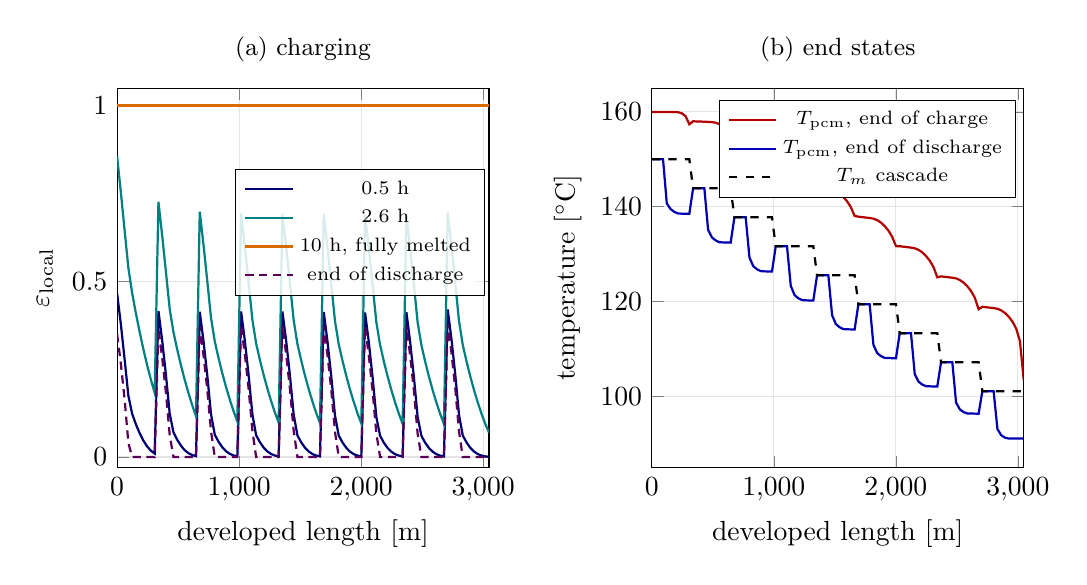
\begin{tikzpicture}
\begin{axis}[width=0.52\linewidth,height=6.4cm,
  xlabel={developed length [m]}, ylabel={$\epsloc$},
  title={\small (a) charging}, ymin=-0.03, ymax=1.05, xmin=0, xmax=3048,
  legend style={font=\scriptsize,at={(0.99,0.62)},anchor=east,fill=white,fill opacity=0.85,draw opacity=1,text opacity=1},
  grid=both, grid style={gray!20}]
\addplot[thick,blue!45!black] coordinates {
(0.0,0.4662) (30.8,0.3782) (61.6,0.2781) (92.4,0.1745) (123.2,0.1233)
(153.9,0.0934) (184.7,0.0679) (215.5,0.0467) (246.3,0.0302) (277.1,0.0181)
(307.9,0.0101) (338.7,0.4160) (369.5,0.3317) (400.2,0.2335) (431.0,0.1236)
(461.8,0.0706) (492.6,0.0492) (523.4,0.0322) (554.2,0.0195) (585.0,0.0109)
(615.8,0.0057) (646.5,0.0026) (677.3,0.4134) (708.1,0.3301) (738.9,0.2326)
(769.7,0.1216) (800.5,0.0636) (831.3,0.0436) (862.1,0.0279) (892.8,0.0166)
(923.6,0.0091) (954.4,0.0046) (985.2,0.0021) (1016.0,0.4143) (1046.8,0.3312)
(1077.6,0.2337) (1108.4,0.1222) (1139.2,0.0622) (1169.9,0.0424) (1200.7,0.0270)
(1231.5,0.0159) (1262.3,0.0087) (1293.1,0.0043) (1323.9,0.0019) (1354.7,0.4141)
(1385.5,0.3306) (1416.2,0.2327) (1447.0,0.1208) (1477.8,0.0616) (1508.6,0.0420)
(1539.4,0.0266) (1570.2,0.0157) (1601.0,0.0085) (1631.8,0.0042) (1662.5,0.0019)
(1693.3,0.4127) (1724.1,0.3287) (1754.9,0.2302) (1785.7,0.1176) (1816.5,0.0610)
(1847.3,0.0414) (1878.1,0.0262) (1908.8,0.0154) (1939.6,0.0083) (1970.4,0.0041)
(2001.2,0.0018) (2032.0,0.4114) (2062.8,0.3269) (2093.6,0.2276) (2124.4,0.1143)
(2155.2,0.0604) (2185.9,0.0409) (2216.7,0.0258) (2247.5,0.0151) (2278.3,0.0082)
(2309.1,0.0040) (2339.9,0.0018) (2370.7,0.4125) (2401.5,0.3277) (2432.2,0.2278)
(2463.0,0.1135) (2493.8,0.0603) (2524.6,0.0408) (2555.4,0.0257) (2586.2,0.0151)
(2617.0,0.0081) (2647.8,0.0040) (2678.5,0.0018) (2709.3,0.4201) (2740.1,0.3357)
(2770.9,0.2359) (2801.7,0.1208) (2832.5,0.0614) (2863.3,0.0418) (2894.1,0.0264)
(2924.8,0.0156) (2955.6,0.0085) (2986.4,0.0042) (3017.2,0.0019) (3048.0,0.0007)};
\addlegendentry{0.5 h}
\addplot[thick,teal] coordinates {
(0.0,0.8562) (30.8,0.7536) (61.6,0.6449) (92.4,0.5383) (123.2,0.4671)
(153.9,0.4093) (184.7,0.3559) (215.5,0.3066) (246.3,0.2612) (277.1,0.2202)
(307.9,0.1825) (338.7,0.7265) (369.5,0.6304) (400.2,0.5265) (431.0,0.4215)
(461.8,0.3556) (492.6,0.3063) (523.4,0.2609) (554.2,0.2198) (585.0,0.1821)
(615.8,0.1476) (646.5,0.1164) (677.3,0.6984) (708.1,0.6040) (738.9,0.5013)
(769.7,0.3959) (800.5,0.3290) (831.3,0.2818) (862.1,0.2386) (892.8,0.1993)
(923.6,0.1633) (954.4,0.1305) (985.2,0.1013) (1016.0,0.6941) (1046.8,0.5999)
(1077.6,0.4972) (1108.4,0.3914) (1139.2,0.3236) (1169.9,0.2768) (1200.7,0.2340)
(1231.5,0.1949) (1262.3,0.1592) (1293.1,0.1268) (1323.9,0.0980) (1354.7,0.6928)
(1385.5,0.5983) (1416.2,0.4953) (1447.0,0.3892) (1477.8,0.3219) (1508.6,0.2751)
(1539.4,0.2323) (1570.2,0.1933) (1601.0,0.1577) (1631.8,0.1254) (1662.5,0.0967)
(1693.3,0.6912) (1724.1,0.5962) (1754.9,0.4927) (1785.7,0.3865) (1816.5,0.3205)
(1847.3,0.2737) (1878.1,0.2310) (1908.8,0.1920) (1939.6,0.1564) (1970.4,0.1242)
(2001.2,0.0955) (2032.0,0.6897) (2062.8,0.5943) (2093.6,0.4902) (2124.4,0.3838)
(2155.2,0.3192) (2185.9,0.2724) (2216.7,0.2297) (2247.5,0.1908) (2278.3,0.1552)
(2309.1,0.1231) (2339.9,0.0945) (2370.7,0.6902) (2401.5,0.5945) (2432.2,0.4899)
(2463.0,0.3828) (2493.8,0.3185) (2524.6,0.2716) (2555.4,0.2290) (2586.2,0.1901)
(2617.0,0.1545) (2647.8,0.1224) (2678.5,0.0939) (2709.3,0.6960) (2740.1,0.6005)
(2770.9,0.4958) (2801.7,0.3872) (2832.5,0.3196) (2863.3,0.2726) (2894.1,0.2298)
(2924.8,0.1908) (2955.6,0.1551) (2986.4,0.1230) (3017.2,0.0944) (3048.0,0.0696)};
\addlegendentry{2.6 h}
\addplot[very thick,orange!85!black] coordinates {(0,1) (3048,1)};
\addlegendentry{10 h, fully melted}
\addplot[thick,densely dashed,violet!70!black] coordinates {
(0.0,0.3500) (30.8,0.2655) (61.6,0.1643) (92.4,0.0402) (123.2,0.0000)
(153.9,0.0000) (184.7,0.0000) (215.5,0.0000) (246.3,0.0000) (277.1,0.0000)
(307.9,0.0000) (338.7,0.3649) (369.5,0.2823) (400.2,0.1836) (431.0,0.0630)
(461.8,0.0000) (492.6,0.0000) (523.4,0.0000) (554.2,0.0000) (585.0,0.0000)
(615.8,0.0000) (646.5,0.0000) (677.3,0.3719) (708.1,0.2901) (738.9,0.1924)
(769.7,0.0731) (800.5,0.0000) (831.3,0.0000) (862.1,0.0000) (892.8,0.0000)
(923.6,0.0000) (954.4,0.0000) (985.2,0.0000) (1016.0,0.3745) (1046.8,0.2928)
(1077.6,0.1953) (1108.4,0.0761) (1139.2,0.0000) (1169.9,0.0000) (1200.7,0.0000)
(1231.5,0.0000) (1262.3,0.0000) (1293.1,0.0000) (1323.9,0.0000) (1354.7,0.3746)
(1385.5,0.2925) (1416.2,0.1946) (1447.0,0.0748) (1477.8,0.0000) (1508.6,0.0000)
(1539.4,0.0000) (1570.2,0.0000) (1601.0,0.0000) (1631.8,0.0000) (1662.5,0.0000)
(1693.3,0.3733) (1724.1,0.2907) (1754.9,0.1920) (1785.7,0.0712) (1816.5,0.0000)
(1847.3,0.0000) (1878.1,0.0000) (1908.8,0.0000) (1939.6,0.0000) (1970.4,0.0000)
(2001.2,0.0000) (2032.0,0.3720) (2062.8,0.2889) (2093.6,0.1894) (2124.4,0.0673)
(2155.2,0.0000) (2185.9,0.0000) (2216.7,0.0000) (2247.5,0.0000) (2278.3,0.0000)
(2309.1,0.0000) (2339.9,0.0000) (2370.7,0.3729) (2401.5,0.2895) (2432.2,0.1893)
(2463.0,0.0660) (2493.8,0.0000) (2524.6,0.0000) (2555.4,0.0000) (2586.2,0.0000)
(2617.0,0.0000) (2647.8,0.0000) (2678.5,0.0000) (2709.3,0.3799) (2740.1,0.2969)
(2770.9,0.1971) (2801.7,0.0737) (2832.5,0.0000) (2863.3,0.0000) (2894.1,0.0000)
(2924.8,0.0000) (2955.6,0.0000) (2986.4,0.0000) (3017.2,0.0000) (3048.0,0.0000)};
\addlegendentry{end of discharge}
\end{axis}
\begin{axis}[width=0.52\linewidth,height=6.4cm,at={(0.56\linewidth,0)},
  xlabel={developed length [m]}, ylabel={temperature [\si{\celsius}]},
  title={\small (b) end states}, ymin=85, ymax=165, xmin=0, xmax=3048,
  legend style={font=\scriptsize,at={(0.98,0.97)},anchor=north east},
  grid=both, grid style={gray!20}]
\addplot[thick,red!70!black] coordinates {
(0.0,160.0000) (30.8,160.0000) (61.6,160.0000) (92.4,160.0000) (123.2,159.9996)
(153.9,159.9973) (184.7,159.9859) (215.5,159.9346) (246.3,159.6928) (277.1,159.1050)
(307.9,157.3940) (338.7,158.0194) (369.5,157.9898) (400.2,157.9602) (431.0,157.9301)
(461.8,157.8957) (492.6,157.8441) (523.4,157.7264) (554.2,157.4005) (585.0,156.8359)
(615.8,155.9434) (646.5,154.3090) (677.3,154.4368) (708.1,154.3757) (738.9,154.3148)
(769.7,154.2524) (800.5,154.1776) (831.3,154.0485) (862.1,153.7300) (892.8,153.1955)
(923.6,152.4286) (954.4,151.3538) (985.2,149.6631) (1016.0,149.5682) (1046.8,149.4866)
(1077.6,149.4053) (1108.4,149.3216) (1139.2,149.2162) (1169.9,148.9965) (1200.7,148.5635)
(1231.5,147.9183) (1262.3,147.0444) (1293.1,145.8705) (1323.9,144.1143) (1354.7,143.9387)
(1385.5,143.8470) (1416.2,143.7556) (1447.0,143.6612) (1477.8,143.5376) (1508.6,143.2594)
(1539.4,142.7691) (1570.2,142.0673) (1601.0,141.1358) (1631.8,139.8990) (1662.5,138.0570)
(1693.3,137.9112) (1724.1,137.8157) (1754.9,137.7207) (1785.7,137.6219) (1816.5,137.4882)
(1847.3,137.1790) (1878.1,136.6576) (1908.8,135.9231) (1939.6,134.9542) (1970.4,133.6626)
(2001.2,131.6957) (2032.0,131.6741) (2062.8,131.5783) (2093.6,131.4829) (2124.4,131.3832)
(2155.2,131.2438) (2185.9,130.9166) (2216.7,130.3759) (2247.5,129.6193) (2278.3,128.6198)
(2309.1,127.2688) (2339.9,125.1204) (2370.7,125.3191) (2401.5,125.2248) (2432.2,125.1309)
(2463.0,125.0326) (2493.8,124.8911) (2524.6,124.5543) (2555.4,124.0023) (2586.2,123.2304)
(2617.0,122.2041) (2647.8,120.7861) (2678.5,118.3923) (2709.3,118.9079) (2740.1,118.8161)
(2770.9,118.7248) (2801.7,118.6293) (2832.5,118.4919) (2863.3,118.1566) (2894.1,117.6041)
(2924.8,116.8275) (2955.6,115.7844) (2986.4,114.3064) (3017.2,111.6497) (3048.0,103.5006)};
\addlegendentry{$\Tpcm$, end of charge}
\addplot[thick,blue!70!black] coordinates {
(0.0,150.0000) (30.8,150.0000) (61.6,150.0000) (92.4,150.0000) (123.2,140.7038)
(153.9,139.5281) (184.7,138.9149) (215.5,138.5798) (246.3,138.5421) (277.1,138.5194)
(307.9,138.4989) (338.7,143.8889) (369.5,143.8889) (400.2,143.8889) (431.0,143.8889)
(461.8,135.1113) (492.6,133.5472) (523.4,132.8973) (554.2,132.5236) (585.0,132.4761)
(615.8,132.4531) (646.5,132.4329) (677.3,137.7778) (708.1,137.7778) (738.9,137.7778)
(769.7,137.7778) (800.5,129.3280) (831.3,127.4865) (862.1,126.8195) (892.8,126.4306)
(923.6,126.3774) (954.4,126.3543) (985.2,126.3341) (1016.0,131.6667) (1046.8,131.6667)
(1077.6,131.6667) (1108.4,131.6667) (1139.2,123.3137) (1169.9,121.3806) (1200.7,120.7091)
(1231.5,120.3179) (1262.3,120.2647) (1293.1,120.2417) (1323.9,120.2216) (1354.7,125.5556)
(1385.5,125.5556) (1416.2,125.5556) (1447.0,125.5556) (1477.8,117.1304) (1508.6,115.2582)
(1539.4,114.5914) (1570.2,114.2078) (1601.0,114.1591) (1631.8,114.1366) (1662.5,114.1167)
(1693.3,119.4444) (1724.1,119.4444) (1754.9,119.4444) (1785.7,119.4444) (1816.5,110.8811)
(1847.3,109.1545) (1878.1,108.5015) (1908.8,108.1357) (1939.6,108.0943) (1970.4,108.0728)
(2001.2,108.0538) (2032.0,113.3333) (2062.8,113.3333) (2093.6,113.3333) (2124.4,113.3333)
(2155.2,104.6835) (2185.9,103.1275) (2216.7,102.4994) (2247.5,102.1646) (2278.3,102.1318)
(2309.1,102.1128) (2339.9,102.0961) (2370.7,107.2222) (2401.5,107.2222) (2432.2,107.2222)
(2463.0,107.2222) (2493.8,98.6873) (2524.6,97.2845) (2555.4,96.6973) (2586.2,96.4137)
(2617.0,96.3910) (2647.8,96.3775) (2678.5,96.3659) (2709.3,101.1111) (2740.1,101.1111)
(2770.9,101.1111) (2801.7,101.1111) (2832.5,93.1500) (2863.3,91.8351) (2894.1,91.3174)
(2924.8,91.1208) (2955.6,91.1127) (2986.4,91.1111) (3017.2,91.1111) (3048.0,91.1111)};
\addlegendentry{$\Tpcm$, end of discharge}
\addplot[thick,black,dashed] coordinates {
(0.0,150.0000) (30.8,150.0000) (61.6,150.0000) (92.4,150.0000) (123.2,150.0000)
(153.9,150.0000) (184.7,150.0000) (215.5,150.0000) (246.3,150.0000) (277.1,150.0000)
(307.9,150.0000) (338.7,143.8889) (369.5,143.8889) (400.2,143.8889) (431.0,143.8889)
(461.8,143.8889) (492.6,143.8889) (523.4,143.8889) (554.2,143.8889) (585.0,143.8889)
(615.8,143.8889) (646.5,143.8889) (677.3,137.7778) (708.1,137.7778) (738.9,137.7778)
(769.7,137.7778) (800.5,137.7778) (831.3,137.7778) (862.1,137.7778) (892.8,137.7778)
(923.6,137.7778) (954.4,137.7778) (985.2,137.7778) (1016.0,131.6667) (1046.8,131.6667)
(1077.6,131.6667) (1108.4,131.6667) (1139.2,131.6667) (1169.9,131.6667) (1200.7,131.6667)
(1231.5,131.6667) (1262.3,131.6667) (1293.1,131.6667) (1323.9,131.6667) (1354.7,125.5556)
(1385.5,125.5556) (1416.2,125.5556) (1447.0,125.5556) (1477.8,125.5556) (1508.6,125.5556)
(1539.4,125.5556) (1570.2,125.5556) (1601.0,125.5556) (1631.8,125.5556) (1662.5,125.5556)
(1693.3,119.4444) (1724.1,119.4444) (1754.9,119.4444) (1785.7,119.4444) (1816.5,119.4444)
(1847.3,119.4444) (1878.1,119.4444) (1908.8,119.4444) (1939.6,119.4444) (1970.4,119.4444)
(2001.2,119.4444) (2032.0,113.3333) (2062.8,113.3333) (2093.6,113.3333) (2124.4,113.3333)
(2155.2,113.3333) (2185.9,113.3333) (2216.7,113.3333) (2247.5,113.3333) (2278.3,113.3333)
(2309.1,113.3333) (2339.9,113.3333) (2370.7,107.2222) (2401.5,107.2222) (2432.2,107.2222)
(2463.0,107.2222) (2493.8,107.2222) (2524.6,107.2222) (2555.4,107.2222) (2586.2,107.2222)
(2617.0,107.2222) (2647.8,107.2222) (2678.5,107.2222) (2709.3,101.1111) (2740.1,101.1111)
(2770.9,101.1111) (2801.7,101.1111) (2832.5,101.1111) (2863.3,101.1111) (2894.1,101.1111)
(2924.8,101.1111) (2955.6,101.1111) (2986.4,101.1111) (3017.2,101.1111) (3048.0,101.1111)};
\addlegendentry{$\Tm$ cascade}
\end{axis}
\end{tikzpicture}
\caption{The default case at cyclic steady state. (a) The melted fraction along
the tube during charging; the sawtooth is the cascade, each layer melting
fastest where the water first meets it. (b) The PCM temperature at the end of
each half-cycle against the melting-temperature staircase. Where the solid curve
lies above the dashed line the PCM is superheated liquid; below it, subcooled
solid. \textbf{A model carrying melted area can only ever draw the dashed
line.}}
\label{fig:profiles}
\end{figure}

%=======================================================================
\section{The parameters, and how they are coupled}
\label{sec:params}

This is the section to read before your first sweep. Several parameters do more
than one job, and the second job is usually the one that surprises you.

\begin{figure}[htbp]
\centering
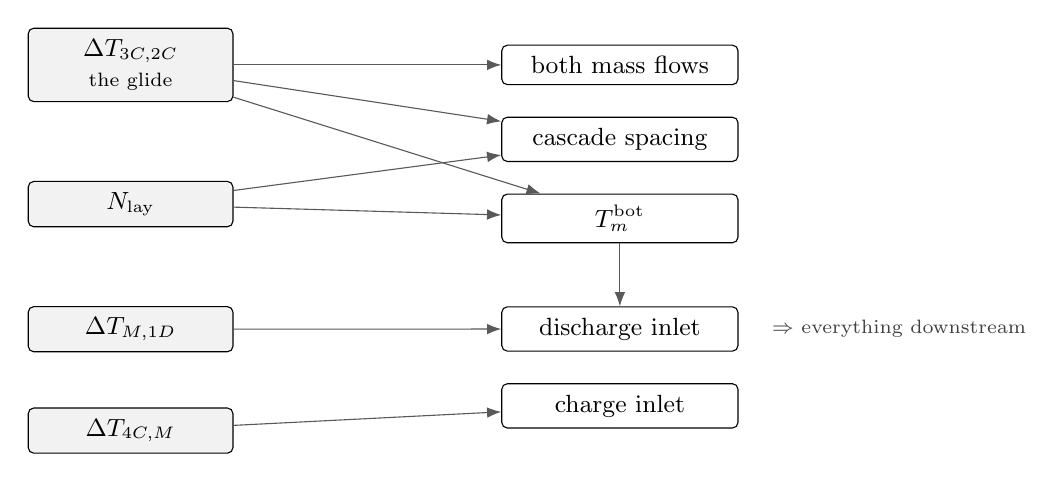
\begin{tikzpicture}[font=\small, node distance=4mm,
  p/.style={draw, rounded corners=2pt, fill=black!5, inner sep=4pt,
            minimum width=26mm, align=center},
  e/.style={draw, rounded corners=2pt, inner sep=4pt, minimum width=30mm,
            align=center},
  a/.style={-{Latex[length=1.8mm]}, gray!70!black}]
\node[p] (glide) {$\Delta T_{3C,2C}$\\\scriptsize the glide};
\node[p, below=10mm of glide] (nlay) {$N_{\mathrm{lay}}$};
\node[p, below=10mm of nlay] (dm1d) {$\Delta T_{M,1D}$};
\node[p, below=7mm of dm1d] (d4cm) {$\Delta T_{4C,M}$};

\node[e, right=34mm of glide] (flow) {both mass flows};
\node[e, below=4mm of flow] (spac) {cascade spacing};
\node[e, below=4mm of spac] (tbot) {$\Tm^{\mathrm{bot}}$};
\node[e, below=8mm of tbot] (din) {discharge inlet};
\node[e, below=4mm of din] (cin) {charge inlet};

\draw[a] (glide) -- (flow);
\draw[a] (glide) -- (spac);
\draw[a] (glide) -- (tbot);
\draw[a] (nlay) -- (spac);
\draw[a] (nlay) -- (tbot);
\draw[a] (tbot) -- (din);
\draw[a] (dm1d) -- (din);
\draw[a] (d4cm) -- (cin);
\node[font=\scriptsize, right=3mm of din, align=left, gray!50!black]
  {$\Rightarrow$ everything downstream};
\end{tikzpicture}
\caption{Parameter couplings. $\Delta T_{4C,M}$ and $\Delta T_{M,1D}$ are the
two \emph{clean} knobs: each moves exactly one inlet and nothing else. The
glide and the layer count each do three jobs.}
\label{fig:couplings}
\end{figure}

\paragraph{The trap.} Change the glide expecting a mass-flow effect and you
have also moved the melting-temperature ladder and, through
Eq.~\eqref{eq:Tmbot}, the discharge inlet. If you want to vary the flow alone,
vary the glide and adjust $\Delta T_{M,1D}$ to hold
$\Tm^{\mathrm{bot}}-\Delta T_{M,1D}$ fixed.

\paragraph{Rate or inventory?}
Every parameter acts on one of two things, and telling them apart is most of
the skill:

\begin{center}
\begin{tabular}{@{}l l l@{}}
\toprule
acts on the \textbf{inventory} & acts on the \textbf{rate} & acts on both \\
\midrule
$\hm$, $\rho$ & $k_s$, $k_l$ & $\Delta T_{3C,2C}$ \\
$V_{\mathrm{well}}$, well depth & fins ($n_f$, $L_f$, $t_f$) & $N_{\mathrm{lay}}$ \\
 & tube radii & $\Tm$ \\
 & $\Delta T_{4C,M}$, $\Delta T_{M,1D}$ & \\
 & window lengths & \\
\bottomrule
\end{tabular}
\end{center}

\textbf{The residual melted fraction at the end of discharge is the
instrument.} If it is near zero, the store empties completely and you are
\emph{inventory} limited: more PCM would help. If it is well above zero, and
particularly if it \emph{rises} when you add wells, you are \emph{rate} limited:
more PCM will not help, and the lever is flow, window length or conductance.

A sweep that moves the deviation a lot and the residual hardly at all is
changing the size of the plant. One that moves the residual is changing its
physics.

\paragraph{Do not tune to zero deviation.}
It is tempting, when a sweep crosses the \SI{1}{\mega\watt} target, to adopt
that parameter value. Resist it. The deviation is the one honestly reported
output of the whole procedure; choosing a parameter so as to zero it converts it
back into a satisfied constraint and throws away the information. Choose
parameters for reasons --- $\Delta T_{M,1D}=\SI{10}{\kelvin}$ is used because it
is symmetric with the charging superheat --- and let the deviation say what it
says.

%=======================================================================
\section{Running it}
\label{sec:running}

In the notebook, \S3.1 is the only cell you need to edit. \code{Case} is a
frozen dataclass, so variants are made by copying:

\begingroup
\small
\noindent\rule{\linewidth}{0.4pt}
\begin{verbatim}
  case = CASE.with_(h_m = 180_000.0,      # J/kg, not kJ/kg
                    N_lay = 12)
  validate_case(case)
  css = simulate_css_corrected(case, record=True, n_cycles=300)
  css_report(case, css)
\end{verbatim}
\vspace{-1.2em}
\noindent\rule{\linewidth}{0.4pt}
\endgroup
\medskip

Four things that will otherwise cost you an afternoon:

\begin{enumerate}\itemsep3pt
\item \textbf{Units are SI base units.} $\hm$ is in \si{\joule\per\kilogram}, so
  \SI{180}{\kilo\joule\per\kilogram} is \code{180\_000.0}. Writing \code{180}
  gives a store with essentially no capacity, and no error.

\item \textbf{Edit \S3.1, not the model cell.} Rewriting a default inside the
  \code{\%\%writefile} cell changes the file on disk but not the module already
  imported, so the old value is used and the old answer is reported without
  complaint.

\item \textbf{Watch the convergence banner.} Cycles to convergence grow with the
  well count. The default limit of 80 is comfortable at the design point and
  \emph{not} comfortable at, say, $\hm=\SI{180}{\kilo\joule\per\kilogram}$,
  which needs 117. If you see \code{*** NOT CONVERGED ***}, raise
  \code{n\_cycles}; nothing below that line means anything until you do.

\item \textbf{Run \code{validate\_case} every time.} It does not check that the
  model is right --- that is settled elsewhere --- but that \emph{your
  parameters} are consistent: layer boundaries falling inside segments, an inlet
  on the wrong side of the cascade, an approach narrower than one layer width.
\end{enumerate}

%=======================================================================
\section{What the model does not contain}
\label{sec:limits}

A parametric study can wander into the region where one of these dominates, so
they are worth knowing by name.

\begin{enumerate}\itemsep3pt
\item \textbf{No ground heat loss} (H6). The store is adiabatic, so
  $\eta_{\mathrm{storage}}\equiv1$ at cyclic steady state \emph{by
  construction}. No sweep can produce a storage loss, and you should not read
  the perfect round trip as a result.

\item \textbf{H3 is saturated.} At the design point the melt fronts of
  neighbouring tubes are in contact over \SI{99}{\percent} of the exchanger, so
  the annular conduction resistance is being evaluated at the exact limit of its
  validity. Sweeps that \emph{increase} melting --- more fins, higher $k$, longer
  charging --- go further into that region, not out of it.

\item \textbf{H9 is unquantified and not small.} The two legs of a hairpin are
  up to \SI{48.9}{\kelvin} apart at the wellhead and are assumed perfectly
  insulated from one another. The neglected leak is of order \SI{25}{\percent}
  of the useful duty.

\item \textbf{No validation against experiment} or against a
  higher-fidelity model. Energy closure is structural: it shows the
  implementation is self-consistent, not that it is right. This is the largest
  open item.

\item \textbf{Idealised cycles.} The compressions and expansions carry no
  isentropic efficiency, so the COP and $\eta_{\mathrm{ORC}}$ are optimistic.

\item \textbf{No volume change on melting}, and the melt-front shape around the
  fins is not modelled.
\end{enumerate}

A deviation of a few per cent sits \emph{inside} the uncertainty of items
1--3. Use it to compare cases, not as an absolute.

\vspace{1em}
\noindent\rule{\linewidth}{0.4pt}

\begin{center}
\begin{tabular}{@{}l l@{}}
\multicolumn{2}{@{}l}{\textbf{Where the rest is}}\\[3pt]
\code{P2H2P\_model.ipynb} & this document, executable \\
\code{P2H2P\_verification.ipynb} & fixtures, regression checks, version history \\
\code{DESIGN\_NOTES.md} & why each superseded approach was superseded \\
project report & the full model statement, equation by equation \\
manuscript & the formulation and its numerics, for publication \\
\end{tabular}
\end{center}

\end{document}
